%%%%%%%%%%%%%%%%%%%%%%%%%%%%%%%%%%%%%%%%%%%%%%%%%%
% Basic setup. Most papers should leave these options alone.
\documentclass[a4paper,fleqn,usenatbib]{mnras}

% MNRAS is set in Times font. If you don't have this installed (most LaTeX
% installations will be fine) or prefer the old Computer Modern fonts, comment
% out the following line
\usepackage{newtxtext,newtxmath}
% Depending on your LaTeX fonts installation, you might get better results with one of these:
%\usepackage{mathptmx}
%\usepackage{txfonts}

% Use vector fonts, so it zooms properly in on-screen viewing software
% Don't change these lines unless you know what you are doing
\usepackage[T1]{fontenc}
\usepackage{ae,aecompl}


%%%%% AUTHORS - PLACE YOUR OWN PACKAGES HERE %%%%%

% Only include extra packages if you really need them. Common packages are:
\usepackage{graphicx}	% Including figure files
\usepackage{amsmath}	% Advanced maths commands
\usepackage{amssymb}	% Extra maths symbols

%%%%%%%%%%%%%%%%%%%%%%%%%%%%%%%%%%%%%%%%%%%%%%%%%%

%%%%% AUTHORS - PLACE YOUR OWN COMMANDS HERE %%%%%

% Please keep new commands to a minimum, and use \newcommand not \def to avoid
% overwriting existing commands. Example:
%\newcommand{\pcm}{\,cm$^{-2}$}	% per cm-squared
\newcommand{\name}{SN-BHM}
\newcommand{\myemail}{samuelreay@gmail.com}
\newcommand\abs[1]{\left|#1\right|}
\newcommand {\etal} {\emph{~et~al.} }
\newcommand{\cov}{\mathcal{C}^{-1}}
\newcommand{\green}{\color{green}}
\newcommand{\blue}{\color{blue}}
\newcommand{\red}{\color{red}}

\newcommand{\kmsmpc}{{\rm km}\,{\rm s}^{-1}\,{\rm Mpc}^{-1}}

\defcitealias{Guy2010}{G10}
\defcitealias{Chotard2011}{C11}
\defcitealias{Rubin2015}{R15}	
\defcitealias{Scolnic2016}{SK16}	 
\newcommand{\gten}{\citetalias{Guy2010}}
\newcommand{\celeven}{\citetalias{Chotard2011}}
\newcommand{\rubin}{\citetalias{Rubin2015}}
\newcommand{\sk}{\citetalias{Scolnic2016}}
\newcommand{\angstrom}{\mbox{\normalfont\AA}}

\graphicspath{ {./figures/} }
%%%%%%%%%%%%%%%%%%%%%%%%%%%%%%%%%%%%%%%%%%%%%%%%%%

%%%%%%%%%%%%%%%%%%% TITLE PAGE %%%%%%%%%%%%%%%%%%%

% Title of the paper, and the short title which is used in the headers.
% Keep the title short and informative.
\title[\name]{\name: A hierarchical Bayesian model for Supernova Cosmology}

% The list of authors, and the short list which is used in the headers.
% If you need two or more lines of authors, add an extra line using \newauthor
\author[S. R. Hinton et al.]{
	Samuel R. Hinton,$^{1,2}$\thanks{E-mail: samuelreay@gmail.com}
	Alex G. Kim,$^{3}$
	Tamara M. Davis$^{1,2}$
	\\
	% List of institutions
	$^{1}$School of Mathematics and Physics, The University of Queensland, Brisbane, QLD 4072, Australia\\
	$^{2}$ARC Centre of Excellence for All-sky Astrophysics (CAASTRO)\\
	$^{3}$Physics Division, Lawrence Berkeley National Laboratory, 1 Cyclotron Road, Berkeley, CA 94720, USA
}

% These dates will be filled out by the publisher
\date{Accepted XXX. Received YYY; in original form ZZZ}

% Enter the current year, for the copyright statements etc.
\pubyear{2017}

% Don't change these lines
\begin{document}
\label{firstpage}
\pagerange{\pageref{firstpage}--\pageref{lastpage}}
\maketitle











% Abstract of the paper
\begin{abstract}
Abstract Abstract Abstract Abstract Abstract Abstract Abstract Abstract Abstract Abstract
Abstract Abstract Abstract Abstract Abstract Abstract Abstract Abstract Abstract Abstract
Abstract Abstract Abstract Abstract Abstract Abstract Abstract Abstract Abstract Abstract
Abstract Abstract Abstract Abstract Abstract Abstract Abstract Abstract Abstract Abstract
Abstract Abstract Abstract Abstract Abstract Abstract Abstract Abstract Abstract Abstract
Abstract Abstract Abstract Abstract Abstract Abstract Abstract Abstract Abstract Abstract
\end{abstract}

% Select between one and six entries from the list of approved keywords.
% Don't make up new ones.
\begin{keywords}
keyword1 -- keyword2 -- keyword3
\end{keywords}









%%%%%%%%%%%%%%%%% BODY OF PAPER %%%%%%%%%%%%%%%%%%

\section{Introduction}

Almost two decades have passed since the discovery of the accelerating universe \citep{Riess1998, Perlmutter1999}. Since that time, of the number of observed Type Ia supernovae (SN Ia) have increased by more than an order of magnitude thanks to modern surveys at both low redshift \citep{Bailey2008, Freedman2009, Hicken2009,  Contreras2010, Conley2011}, and higher redshift \citep{Astier2006, Wood-Vasey2007, Balland2009, Amanullah2010}. Cosmological analysis of these supernova samples \citep{Kowalski2008, Conley2011, Suzuki2012, Betoule2014, Rest2014} have been combined with complimentary probes of large scale structure \citep{Alam2017} and the CMB \citep{Hinshaw2013, PlanckCollaboration2013}, and yet, despite these prodigious efforts, the nature of dark energy remains an unsolved mystery.

In attempts to tease out the nature of dark energy, currently running and planned surveys are once again ramping up their statistical power. The Dark Energy Survey \citep[DES,][]{Bernstein2012, Abbott2016} will be observing thousands of Type Ia supernova, attaining both spectroscopic and photometric confirmation. The Large Synoptic Survey Telescope \citep[LSST,][]{Ivezic2008, LSSTScienceCollaboration2009} will produce scores of thousands of photometrically classified supernovae. Such increased statistical power demands a similarly increased fidelity and flexibility in modelling the supernovae for cosmological purposes, as systematic uncertainty will prove to be the limiting factor in our analyses.

As such, staggering effort is being put into developing more sophisticated supernovae analyses. \citet{Scolnic2016} and \citet{Kessler2017} explore sophisticated simulation corrections to traditional analyses. Approximate Bayesian computation methods also make use of simulations, trading traditional likelihoods and analytic approximations for more robust models with only the cost of increased computational time \citep{Weyant2013, Jennings2016}. Hierarchical Bayesian Models abound \citep{Mandel2009, March2011, March2014, Rubin2015, Shariff2016, Roberts2017}, however often face difficulties finding sufficient analytic approximations for complicated effects such as Malmquist bias.


In this paper, we lay out a new hierarchical model that extends on past work. Section \ref{sec:review} is dedicated to a quick review of the supernovae cosmology. In Section \ref{sec:method} we outline our methodology. Model verification on simulated datasets is given in Section \ref{sec:verification}. Forecasts for the impending DES three year spectroscopic supernova survey are contain in Section \ref{sec:forecast}. Section \ref{sec:sys} investigates the effect of various systematics on our model, and Section \ref{sec:details} provides details on potential areas of improvement and unsuccessful methodologies.









\section{Review}
\label{sec:review}

Whilst supernova observations take the form of time-series photometric measurements of brightness in many photometric bands, most analyses do not work from these measurements of apparent magnitude and colour. Instead, most techniques fit these observations of magnitude (along with redshift) to a supernova model, with the most widely used being that of the empirical SALT2 model \citep{Guy2007, Guy2010}. This model is trained separately before fitting the supernovae light curves for the cosmology selected supernova sample \citep{Guy2010, Mosher2014}. The resulting output from the model is, for each supernova, a characterised amplitude $x_0$ (which can be converted into apparent magnitude $m_B = -2.5\log(x_0)$), a stretch term $x_1$ and colour term $c$, along with a covariance matrix describing the uncertainty on these summary statistics. As such, the product at the end is a (redshift dependent) population of $m_B$, $x_1$ and $c$.

The underlying actual supernova population is not as clear cut, and indeed accurately characterising this population, its evolution over redshift and effects from environment is one of the challenges of supernova cosmology. However, given some modelled underlying population that lives in the redshift dependent space $M_B$, $x_1$ and $c$, the introduction of cosmology into the model is simple -- it is encoded in the functional map between those two populations, from apparent magnitude space to absolute magnitude. Specifically, for any given supernova our functional map may take the traditional form:
\begin{equation}
M_B = m_B + \alpha x_1 - \beta c - \mu(z) + \text{corrections},
\end{equation}
where $\alpha$ is the stretch correction \citep{Phillips1993}, and $\beta$ is the colour correction \citep{Tripp1998} that respectively encapsulate the empirical relation that broader and bluer supernovae are brighter. The $\text{corrections}$ term at the end often includes corrections for host galaxy environment, as this has statistically significant effects on supernova properties \citep{Kelly2010, Lampeitl2010, Sullivan2010, DAndrea2011, Gupta2011, Johansson2013, Rigault2013, Uddin2017}. The cosmological term, $\mu(z)$ represents the distance modulus, and is precisely known given cosmological parameters and an input redshift.

\subsection{Traditional Analyses}

Traditional $\chi^2$ analyses such as that found in \citet{Kowalski2008, Conley2011, Betoule2014}, minimise the difference in distance modulus between the cosmologically predicted values $\mu_C$ and the observed distance modulus $\mu_{\rm obs}$, shown respectively below:
\begin{align}
\mu_C &= 5 \log\left[ \frac{(1+z)r}{10} \right]\\
r& =\frac{c}{H_0} \int_0^z \frac{dz'}{\sqrt{ \Omega_m (1+z')^3 + \Omega_k (1 + z')^2 + \Omega_\Lambda (1+z')^{3(1+w)}}} \\
\mu_{\rm obs} &= m_B + \alpha x_1 - \beta c - M_B
\end{align}
The minimising function is then given as
\begin{equation}
\chi^2 = (\mu_{\rm obs} - \mu_C)^\dagger C^{-1} (\mu_{\rm obs} - \mu_C)
\end{equation}
where $C^{-1}$ is an uncertainty matrix which combined the uncertainty from the SALT2 fits, intrinsic dispersion, calibration, dust, peculiar velocity and many other factors (see \citet{Betoule2014} for a review). The benefit this analysis methodology provides is speed - for samples of hundreds of supernova, efficient matrix inversion algorithms allow the likelihood to be evaluated quickly. The speed comes with two costs. Firstly, formulating a $\chi^2$ likelihood requires a loss of model flexibility by building into the model assumptions of uncertainty Gaussianity. Secondly, the computational efficiency is dependent on inverting a covariance matrix with dimensionality linearly proportional to the number of supernovae. As this number increases, the cost of inversion rises quickly, and is not viable for samples with thousands of supernovae.

Selection efficiency, such as the well known Malmquist bias \citep{MalmquistK.G.1922} is accounted for by correcting data. Simulations following survey observational strategies and geometry and used to calculate the expected bias in distance modulus, which is then added onto the observational data.

\subsection{Approximate Bayesian Computation}

To try and escape the limitations of the traditional analysis methodology, several recent methods have adopted Approximate Bayesian Computation, where supernova samples are forward modelled in parameter space and compared to observed distributions. \citet{Weyant2013} provides an introduction into ABC methods for supernova cosmology in the context of the SDSS-II results \citep{Sako2014} and Flat $\Lambda$CDM cosmology, whilst \citet{Jennings2016} demonstrates their \textit{superABC} method on simulated first season Dark Energy Survey samples, described in \citet{Kessler2015}. In both examples, the supernova simulation package SNANA \citep{Kessler2009a} is used to forward model the data at each point in parameter space.

By building the systematic uncertainties and selection effects into the simulation package, there is vastly more freedom in how to treat and model those effects. Data does not need to be corrected, analytic approximations do not need to be applied, we are free to incorporate algorithms which simply cannot be expressed in a tractable likelihood. This freedom comes with a cost -- computation. The classical $\chi^2$ method's most computationally expensive step in a fit is matrix inversion. For ABC methods, we must instead simulate an entire supernova population in its entirety -- drawing from underlying supernova populations, modelling light curves, applying selection effects, fitting light curves and applying data cuts. This is an intensive process. Luckily, efficient sampling algorithms that have walkers which rely on the Markov properties of groups instead of individual walkers, such as Ensemble sampling \citep{Foreman-Mackey2013} allow easy parallelisation of parameter fits, such as used in the BAMBIS framework {\red CITE RACHEL}.

One final benefit of ABC methods is that they can move past the traditional treatment of supernovae with summary statistics ($m_B$, $x_1$ and $c$). \citet{Jennings2016} presents both a metric used to compare forward modelled summary statistic populations (denoted the `Tripp' metric) and a metric directly applicable to the observed supernova light curves themselves, however evaluation of systematic uncertainty was only performed using the Tripp metric.

\subsection{Hierarchical Bayesian Models}

Sitting comfortably between the traditional models simplicity and the complexity of forward modelling lies Hierarchical Bayesian Models. With the introduction of multiple layers in our model, we can add far more flexibility than a traditional analysis whilst still maintaining most of the computational benefits that come from having a tractable likelihood. \citet{Mandel2009} and \citet{Mandel2011} construct a hierarchical model which they apply to the light curve fitting for supernova. \citet{March2011, March2014, Karpenka2015} derive a hierarchical model and simplify it by analytically marginalising over nuisance parameters provide a model which offers increased flexibility with reduced uncertainty over the traditional method. The recent BAHAMAS model \citep{Shariff2016} builds off this and reanalyses the JLA dataset, whilst including extra freedom in the correction factors $\alpha$ and $\beta$, finding evidence for redshift dependence on $\beta$. \citet{Ma2016} also performed a reanalysis of the JLA dataset, finding significant difference in $\alpha$ and $\beta$ values from the original as well. Notably, these methods rely on data that is bias corrected, however the UNITY framework given by \citet{Rubin2015} incorporates selection efficiency analytically in the model, and is applied to the Union 2.1 dataset \citep{Suzuki2012}. The well known BEAMS (Bayesian estimation applied to multiple species) methodology from \citet{Kunz2007} has been extended and applied in several works \citep{Hlozek2012}, mostly lately to include redshift uncertainty for photometric redshift application as zBEAMS \citep{Roberts2017}. 

The flexibility afforded by a hierarchical model allows for investigations into different treatments of underlying populations, rates, redshift distributions, mass corrections and redshift evolution, each of will will be discussed further in the outline of our model below.









\section{Our Method}
\label{sec:method}

We construct our Bayesian Hierarchical Model with several goals in mind: creation of a redshift dependent correlated underlying supernova population, increased treatment of systematics, and analytic correction of selection effects. As this is closest to the UNITY method from \citet[][hereafter denoted \rubin]{Rubin2015}, we follow a similar model scaffold, and construct the model in Stan \citep{Carpenter2017, StanDevelopmentTeam2017} which uses automatic differentiation and the no-U-turn Sampler (NUTS), which is a variant of Hamiltonian Monte Carlo, to efficiently sample high dimensional parameter space.

At the most fundamental level, a supernova analysis is simply a mapping from an underlying population onto an observed population, where cosmology is encoded directly in the mapping function. The difficulty arises in adding sufficient, physically motivated flexibility in both of these populations whilst not adding \textit{too} much flexibility, such that model fitting becomes pathological due to increasing parameter degeneracies within the model.

\subsection{Observed and Latent Population}

Like most of the BHM methods introduced previously, we work from the summary statistics as well, where each observed supernova has an apparent magnitude $\hat{m_B}$, stretch $\hat{x_1}$ and colour $\hat{c}$, with uncertainty $\cov$ on those values. Additionally, each supernova has an observed redshift $\hat{z}$ and a host galaxy mass associated with it, $\hat{m}$. Given machine learning classifiers to type supernovae, we will also have a probability of being a Type Ia, $\hat{p}$.

The first layer of the hierarchy represents the latent population of $m_B$, $x_1$ and $c$. This can be thought of as the `true' values for the supernova, and is normally distributed around the observed values such that 
\begin{equation}
P(m_B, x_1, c|\hat{m_B},\hat{x_1},\hat{c},\cov) = \mathcal{N}(\lbrace m_B, x_1, c \rbrace|\lbrace \hat{m_B},\hat{x_1},\hat{c} \rbrace, \cov).
\end{equation}
As we are focused on the spectroscopically confirmed DES supernovae for this iteration of the method, we assume the observed redshift $\hat{z}$ is the true redshift $z$, and the similarly that the observed mass is the true mass $m$. Whilst the latter is not physically motivated like the redshift measurement, the relatively small contribution of the host galaxy mass to the model makes this an acceptable approximation.

\subsection{Underlying Population}

The underlying supernova population is often treated with two components - a population distribution in colour and stretch, and intrinsic dispersion. Analytic models often treat the colour and stretch populations with a skew normal and normal, respectively, and have them as independent. Intrinsic dispersion is treated in a variety of manners in other models, from representing it simply as (Gaussian) scatter on the absolute magnitude of the supernova population, to correlated multivariate normal scatter on the combined magnitude, stretch and colour distribution. Additionally, redshift drift of populations' mean colour and stretch will introduce a cosmological bias in our fits unless the population possesses similar ability to change as a function of redshift. 

We model the underlying population and intrinsic dispersion together as a redshift dependent multivariate skew normal for each survey. Following {\rubin} we allow the mean colour and stretch to vary over redshift, anchoring four equally spaced redshift nodes spanning the redshift range of each survey, linearly interpolating between the nodes. Both the colour and stretch means are modelled with normal priors. The correlation between the magnitude, stretch and colour populations is represented in a correlation matrix $\rho$, which is treated with an LKJ prior. Skewness is fixed to 0 for the absolute magnitude population, but left free for colour and stretch, with normal priors centered at 0 to draw the skewness to zero if not well constrained by the data. The decision to include skewness on the stretch distribution as well as the colour was motivated by \citet{Scolnic2016}, which found highly asymmetric underlying populations for both colour and stretch, regardless of survey or scatter model adopted.

The width of the population, represented by the vector $\lbrace \sigma_{M_B}, \sigma_{x_1}, \sigma_c \rbrace$ is subject to Cauchy priors, however are sampled in log space for efficiency in sampling close to zero. 


As such, the only constant between survey populations is the absolute magnitude $M_B$, with the skewness, redshift dependent means, width and correlations fit individual for each survey.

On top of the Ia populations, as described above, we also include a simplistic outlier population that also follows {\rubin} (and therefore \citet{Kunz2007}) as a Gaussian mixture; where the mean of the population is fixed to the Ia population, but the population width is set to a width of $\sigma^{\rm outl} = 1$ in $M_B$, $x_1$ and $c$. With the spectroscopic DES sample, the contamination rate is expected to be far too low to actually fit contamination population, however in future works with photometric samples which will suffer from significantly more contamination it will be required that extra degrees of freedom are afforded the outlier population. Proof of concept simulation fits show that an acceptable parameterisation is to represent the typically brighter contaminant population as $\langle M_B^{\rm outl} \rangle = \langle M_B \rangle - \delta_{M_B}^{\rm outl}$, where $\delta_{M_B}^{\rm outl}$ is constrained to be positive, or even to be greater than a small positive number to reduce degeneracy between the two populations. For the purposes of the DES spectroscopic sample which will be dominated by confirmed Type Ia supernovae, $\delta_{M_B}^{\rm outl} =0$. We assume that supernova fall into either population as determined by their observed classification probability $\hat{p}$.


\subsection{Population Map}

\subsubsection{Cosmology}

We formulate our model with three different cosmological parameterisations; Flat $\Lambda$CDM, Flat $w$CDM and standard $\Lambda$CDM. $\Omega_m$ is given the prior $\mathcal{U}(0.05, 0.99)$, $\Omega_\Lambda$ was treated with $\mathcal{U}(0, 1.5)$ and the equation of state $w$ was similarly set to a flat prior $\mathcal{U}(-0.4, -2.0)$. For calculating the distance modulus, we fix $H_0 = 70 \kmsmpc $. 

\subsubsection{Standardisation Parameters}

With increasingly large datasets and more nuanced analyses, the choice of how to handle $\alpha$ and $\beta$ becomes an important consideration when constructing a model. {\rubin} employs a broken linear relationship for both colour and stretch, where different values of $\alpha$ and $\beta$ are adopted depending on whether $x_1$ and $c$ are respectively positive or negative (although the cut could be placed at a location other than 0). \citet{Shariff2016} instead of employing a colour-dependent $\beta$, model $\beta$ as redshift dependent, testing two phenomenological models; $\beta(z) = \beta_0 + \beta_1 z$ and $\beta(z) = \beta_0 + \Delta \beta\left(0.5 + \arctan(100(z - z_t)) / \pi\right)$, where the later effects a rapid but smooth change in $\beta$ at a turnover redshift $z_t$.

We tested two models against simulated supernova sets; $\beta(c) = \beta_0 + \beta_1 c$ and $\beta(z) = \beta_0 + \beta_1 z$. See Section \ref{sec:simdes} for details on simulation generation. We found for both models that non-zero values for $\beta_1$ are preferred (even with constant $\beta$ used in simulation) due to severe degeneracy with selection effects. This degeneracy resulted in a significant bias in cosmology, and so in our final model we continue to adopt the constant $\alpha$ and $\beta$ found in traditional analyses.

\subsubsection{Host Galaxy Environment}

It is now well known that host galaxy environment has a significant effect on supernova properties. The latest sample of over 1300 spectroscopically confirmed Type Ia supernova show $>5\sigma$ evidence for correlation between host mass and luminosity \citep{Uddin2017}. The traditional correction, as employed in analyses such as \citet{Suzuki2012} and \citet{Betoule2014} invoke a step function such that $\Delta M = 0.08 \mathcal{H}(log(M) - 10))$, where $\mathcal{H}$ is the Heaviside step function and $M$ is the galaxy mass in solar masses. The scale of this step function varies from analysis to analysis, with the 0.08 value shown previously sourced from \cite{Sullivan2010} and used in \citet{Betoule2014}. In this work we adopt the model used in {\rubin}, which follows the work from \citet{Rigault2013}, such that we introduce two parameters to incorporate a redshift-dependent host galaxy mass correction:
\begin{equation}
\Delta M = \delta(0) \left[ \frac{1.9\left(1 - \frac{\delta(0)}{\delta(\infty)}\right)  }{0.9 + 10^{0.95z}} + \frac{\delta(0)}{\delta(\infty)}\right]
\end{equation}
We also take flat priors on the parameterisation $\delta(0)$, $\delta(0)/\delta(\infty)$.

\subsubsection{Systematics}
\label{sec:systreat}
The chief difficulty with including systematics in supernova analyses is that the generally occur during the observational pipeline, and have difficult to model effects on the output observations. As such, the normal treatment for systematics is to compute their effect on the supernova summary statistics -- computing the numerical derivatives $\frac{\partial \hat{m_B}}{\partial Z_i}$, $\frac{\partial \hat{x_1}}{\partial Z_i}$, $\frac{\partial \hat{c}}{\partial Z_i}$, where $Z_i$ represents the $i$\textsuperscript{th} systematic.

Assuming that the gradients can be linearly extrapolated -- which is a reasonable approximation for modern surveys with high quality control of systematics -- we can incorporate into our model a deviation from the observed original values by constructing a $(3 \times N_{\rm sys})$ matrix containing the numerical derivatives for the $N_{\rm sys}$ systematics and multiplying it with the row vector containing the offset for each systematic. But scaling the gradient matrix to represent the shift over $1\sigma$ of systematic uncertainty, we can simply enforce a unit normal prior on the systematic row vector to increase computational efficiency.

This method of adjusting the observed summary statistics is used throughout the traditional and BHM analyses, however it is normally constrained to band systematics. That is, each band for each survey has two systematics associated with it - the calibration uncertainty and the filter wavelength uncertainty. We include these in our approach, in addition to including HST Calspec calibration uncertainty, 10 SALT2 model systematic uncertainties, three dust systematics (scale, dust model, and transfer law) and also the systematic peculiar velocity uncertainty. This gives fourteen global systematics shared by all surveys, plus two systematics per band in each survey.

\subsubsection{Selection Effects}

Our treatment of selection effects is to incorporate selection efficiency into our model, rather than relying on simulation-driven data corrections. As such, we need to describe the probability that the events we observe are both drawn from the distribution predicted by the underlying theoretical model \textit{and} that those events, given they happened, are subsequently successfully observed.  To make this extra conditional explicit, we can write the likelihood of the data given an underlying model, $\theta$, \textit{and} that the data are included in our sample, denoted by $S$, as
\begin{align}
\mathcal{L} &= P({\rm data} | \theta, S). \label{eq:like}
\end{align}
As the model so far described in previous sections describes $P(D|\theta)$, and we wish to formulate a function $P(S|{\rm data},\theta)$ that describes the chance of an event being successfully observed, we rearrange the likelihood in terms of those functions and find
\begin{align}
\mathcal{L} &= \frac{P(S|{\rm data},\theta) P({\rm data}|\theta)}{\int P(S | D, \theta) P(D|\theta)\, dD}, \label{eq:main}
\end{align}
where the denominator represents an integral over all potential data. Full derivation of this can be found in Appendix \ref{app:selection}. As $\theta$ represents the vector of all model parameters, and $D$ represents a vector of all observed variables, this is not a trivial integral. Techniques to approximate this integral, such as Monte-Carlo integration or high dimensional Gaussian processes failed to give tractable posterior surfaces that could be sampled efficiently by HMC. We therefore simplify the integral and approximate the selection effects in apparent magnitude and redshift space independently, such that the denominator, denoted now $w$ for simplicity, is given as
\begin{align}
w &= \int  \left[ \int P(S|m_B) P(m_B | z, \theta)\, d m_B \right] P(S|z) P(z|\theta)\, dz. \label{eq:w1}
\end{align}
We apply two further approximations similar to those made in {\rubin} -- that the redshift distribution of the observed supernova reasonably well sample the $P(S|z)P(z|\theta)$ distribution, and that the survey colour and stretch populations can be treated as Gaussian for the purposes of this integral. The population $P(m_B | z, \theta)$ thus becomes $\mathcal{N}(m_B|m_B^*(z), \sigma^*_{m_B})$, where
\begin{align}
m_B^*(z) &= \langle M_B \rangle + \mu(z) - \alpha \langle x_1(z) \rangle + \beta \langle c(z) \rangle \\
\sigma^*_{m_B} &= \sigma_{M_B}^2 + (\alpha \sigma_{x_1})^2 + (\beta \sigma_c)^2 \notag\\ 
&\quad\quad + 2(\beta \sigma_{M_B,c} - \alpha \sigma{m_B,x_1} - \alpha \beta \sigma_{x_1,c})
\end{align}
What then remains is determining the functional form of $P(S|m_B)$. For the treatment of the DES, we find that the error function which smoothly transitions from some constant efficiency down to zero is sufficient. This similar result has been found by many past surveys \citep{Dilday2008, Barbary2010, Perrett2012, Graur2013, Rodney2014} {\red THESE CITATIONS EXACTLY MIRROR RUBIN2015, NOT SURE IF I SHOULD CHANGE THEM}. For our treatment of the low redshift surveys included {\red Introduce which lowz surveys earlier on} we simplify the model fitting and group all low redshift surveys together. This requires a more complicated selection function than the error function used for DES, however is reasonably well fit with a skew normal. The selection functions were fit to apparent magnitude efficiency ratios calculated from SNANA simulations. The DES survey is thus characterised by $\mu_{\rm DES} = 22.3$, $\sigma_{\rm DES} = 0.7$, with the combined low redshift surveys characterised by $\mu_{\rm LowZ} = 14.1$, $\sigma_{\rm LowZ} = 1.36$, $\alpha_{\rm LowZ} = 3.8$.


With the well sampled approximation as specified previously, we can remove the redshift integral in Eq \eqref{eq:w1} and replace it with a correction for each observed supernova. For the error function (DES) and skew normal selection (LowZ) functions respectively, this correction becomes
\begin{align}
w_{\rm DES} &= \Phi^c\left(  \frac{m^*_B - \mu_{\rm DES}}{\sqrt{\sigma^{*2}_{m_B} + \sigma_{\rm DES}^2}}  \right) \\
w_{\rm LowZ} &= 2\mathcal{N}\left( \frac{m_B^* - \mu_{\rm LowZ}}{\sqrt{\sigma^{*2}_{m_B} + \sigma_{\rm LowZ}^2}}\right) \times \notag\\
&\quad\quad \Phi\left(  \frac{{\rm sign}(\alpha_{\rm LowZ})(m_B^* - \mu_{\rm LowZ})}{\frac{\sigma_{m_B}^{*2} + \sigma^2_{\rm LowZ}}{\sigma^2_{\rm LowZ}} \sqrt{\frac{\sigma^2_{\rm LowZ}}{\alpha^2_{\rm LowZ}} + \frac{\sigma_{m_B}^{*2} \sigma^2_{\rm LowZ}}{\sigma_{m_B}^{*2} + \sigma^2_{\rm LowZ}}} }\right),
\end{align}
where $\Phi$ represents the normal CDF function, and $\Phi^c$ the complimentary CDF.








\section{Model Verification}
\label{sec:verification}

In order to verify our model we run it through several tests. First, we validate on toy models, verifying that there is not significant cosmological bias in data sets more constraining than the DES spectroscopic sample. We then also generate 

\subsection{Applied to Toy Spectroscopic Data}
\label{sec:toy}

We generate simple toy data to validate the basic premise of the model. For both DES and LowZ data we draw from an underlying $M_B$, $x_1$, $c$ population and translate into apparent magnitude space using $\Omega_m = 0.3$, $\alpha= 0.14$ and $\beta = 3.1$. Masses are randomly drawn from the interval 0 to 1, and a mass correction with $\delta(0) = 0.08$ and $\delta(0)/\delta(\infty) =0.5$ included. Independent observational errors of $0.04$, $0.2$, $0.03$ on $m_B$, $x_1$ and $c$ (following the mean uncertainty for DES SNANA simulations) are added to create the observables. The results are then passed through the selection effects, where each supernova is only selected based on $P(S|m_B)$, using a skew normal function for the LowZ supernovae and error function for the DES-like supernovae. We draw from each survey simulation until we have 300 LowZ supernovae and 700 DES-like supernovae, representing a statistical sample of greater power than the estimated 250 supernovae for the DES spectroscopic analysis.

The above represents one realisation of data. We test three models (Flat $\Lambda$CDM, Flat $w$CDM, $\Lambda$CDM) with 300 realisations and find recovery of underlying cosmology without significant bias. Combined posterior surfaces of 22 realisations for Flat $wCDM$ fits are shown in Figure \ref{fig:simple_w}.


%\begin{figure}
%	\begin{center}
%		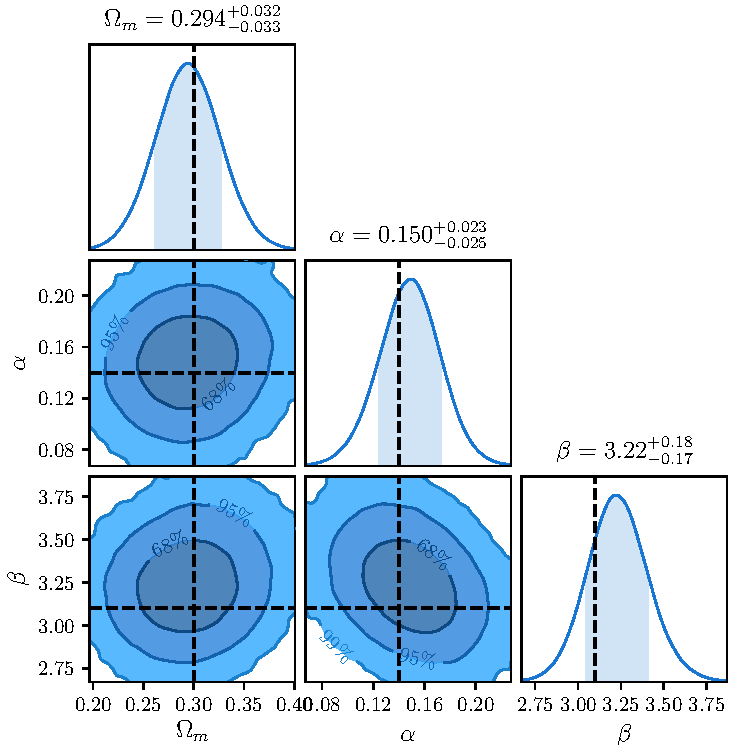
\includegraphics[width=\columnwidth]{approximate_simple_test_cosmo.pdf}
%	\end{center}
%	\caption{Posterior surfaces for 22 realisations of supernova data with the Flat $\Lambda$CDM model.}
%	\label{fig:simple_om}
%\end{figure}
\begin{figure}
	\begin{center}
		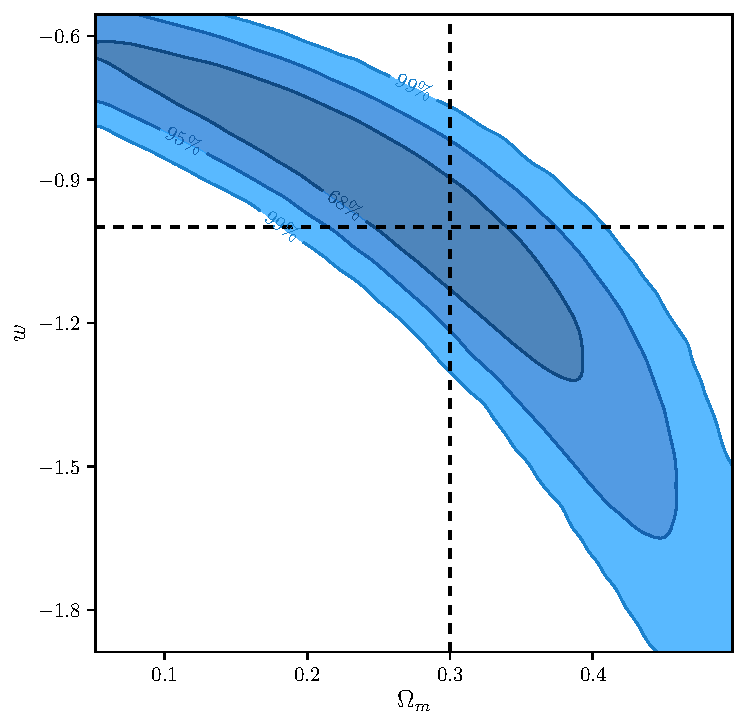
\includegraphics[width=\columnwidth]{approximate_simple_test_w_cosmo.pdf}
	\end{center}
	\caption{Posterior surfaces for 22 realisations of supernova data with the Flat $w$CDM model.}
	\label{fig:simple_w}
\end{figure}
%\begin{figure}
%	\begin{center}
%		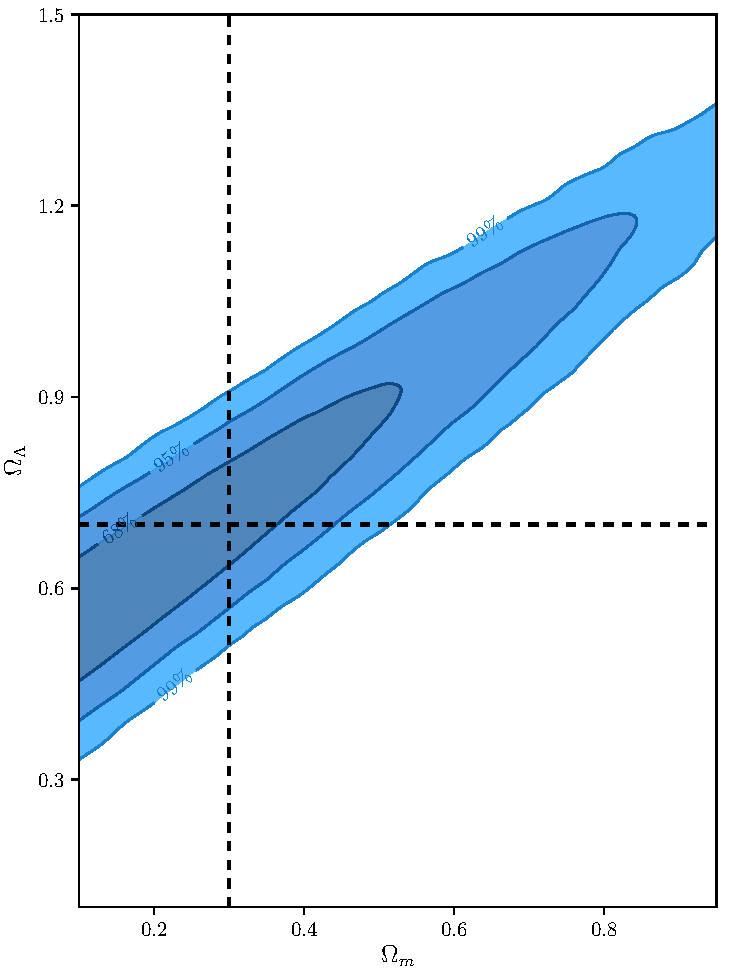
\includegraphics[width=\columnwidth]{approximate_simple_test_ol_cosmo.pdf}
%	\end{center}
%	\caption{Posterior surfaces for 22 realisations of supernova data with the $\Lambda$CDM model.}
%	\label{fig:simple_ol}
%\end{figure}


\subsection{DES SN data validation}
\label{sec:simdes}


Early analyses often treated intrinsic dispersion simply as scatter in the underlying absolute magnitude of the underlying population, but recent analyses require more a more sophisticated approach. In our development of this model and tests of intrinsic dispersion, we analyse the effects of two different scatter models. The first model is the \citet[][hereafter denoted the {\gten} scatter model]{Guy2010}, which models intrinsic scatter with a 70\% contribution from coherent variation and 30\% from chromatic variation. The second model, denoted the {\celeven} model is sourced from \citet{Chotard2011} and has variation with 25\% contribution from coherent scatter and 75\% from chromatic variation. We also test a `Combined' smear model, which is simply to draw equal samples from the {\celeven} and {\gten} models. It is against this combined sample that we wish to rigorously validate our model.

Simulations (using the SNANA package) follow the observational schedule and observing conditions for the DES and LowZ surveys. In addition to the improvements in the scatter models over the simple data, we also include peculiar velocities for the LowZ sample, and now also include our full treatment of systematics. Additionally, we also simulate two different underlying population -- a Gaussian distribution in colour and stretch, and skewed colour and stretch populations using population values from \citet[][hereafter {\sk}]{Scolnic2016}.

\begin{table}
	\centering
	\caption{Tested population distributions, where the {\sk} LowZ distribution is formed as sum of two bifurcated Gaussians, with the mean and spread of each component given respectively.}
	\label{tab:dist}
	\begin{tabular}{l|llll}
		\hline
		Model & $\langle x_1 \rangle$ & $\sigma_{x_1}$ &  $\langle c \rangle$ & $\sigma_c$  \\
		\hline
		Gaussian LowZ &  $0.0$ & $1.0$ & $0.0$ & $0.1$ \\
		Gaussian DES  &  $0.0$ & $1.0$ & $0.0$ & $0.1$  \\
		{\sk} LowZ    &  $0.55$ \& $-1.5$ & $^{+0.45}_{-1.0}$ \& $^{+0.5}_{-0.5}$ & $-0.055$ & $^{+0.15}_{-0.023}$ \\
		{\sk} DES     & $0.973$ & $^{+0.222}_{1.472}$ & $-0.054$  &  $^{+0.101}_{0.043}$ \\
		\hline
	\end{tabular}
\end{table}

Each realisation of cosmology fitted contains 300 LowZ supernovae, and 250 DES-like supernovae, such that the uncertainties found when combining chains is representative of the uncertainty in the final DES spectroscopic analysis. Combined posterior surfaces for 150 data realisations are shown in Figure \ref{fig:bulk_summary}. Note that we have combined the posteriors for 150 realisations, and so we should expect the size of the uncertainty to be representative of one realisation, but the statistical spread of the final surface should be $\sqrt{150} \approx 12$ times less than a single realisation. Plot summaries for the fits are shown in Figure \ref{fig:bulk_summary}, and the parameter bounds are listed in Table \ref{tab:bulk_summary}. The results indicate changes in the underlying population can effect significant changes in the recovered standardisation parameters $\alpha$ and $\beta$, however do not appear to have a significant effect on recovered cosmology. Whilst the combined sample (on which the selection function was fit) shows no significant bias (as expected), the {\celeven} and {\gten} only models show opposite biases in $\Omega_m$. Cosmological bias is detected with $\approx 3.0\sigma$ significance for the {\celeven} model and $\approx 1.7\sigma$ significance for the {\gten} model, indicating that the population and selection effect treatment cannot capture all necessary information to encapsulate the magnitude and chromatic smearing of the supernovae population. However, for the sample size of the DES and LowZ supernova samples (of order 600 supernova), these effects are sub-dominant to the statistical uncertainty, representing at most a deviation of $0.25\sigma$ and, accounting for statistical fluctuations up to $2\sigma$, a minimum bias of $0.08\sigma$ for the {\celeven} model.

\begin{table}
	\centering
	\caption{Parameter summaries shown for 150 realisations of supernovae data, each comprising of 300 LowZ supernovae and 250 DES-like supernovae. Maximum likelihood statistics, with errors quoted to $1\sigma$ (68\% confidence) are reported.}
	\label{tab:bulk_summary}
	\begin{tabular}{ccccc}
		\hline
		Model & $\Omega_m$ & $\alpha$ & $\beta$  \\ 
		\hline
		C11 Gaussian & $0.316^{+0.062}_{-0.064}$ & $0.143^{+0.028}_{-0.027}$ & $2.97^{+0.20}_{-0.19}$  \\ 
		C11 {\sk} & $0.316^{+0.063}_{-0.062}$ & $0.155\pm 0.024$ & $2.77^{+0.26}_{-0.27}$  \\ 
		Combined Gaussian & $0.299^{+0.067}_{-0.060}$ & $0.144^{+0.030}_{-0.028}$ & $3.11^{+0.21}_{-0.22}$  \\ 
		Combined {\sk} & $0.297^{+0.075}_{-0.064}$ & $0.150^{+0.026}_{-0.025}$ & $3.00^{+0.29}_{-0.31}$  \\ 
		G10 Gaussian & $0.290^{+0.070}_{-0.060}$ & $0.145\pm 0.030$ & $3.27\pm 0.23$ \\ 
		G10 {\sk} & $0.290^{+0.079}_{-0.073}$ & $0.147^{+0.026}_{-0.028}$ & $3.26^{+0.34}_{-0.33}$ \\ 
		\hline
	\end{tabular}
\end{table}



\begin{figure}
	\begin{center}
		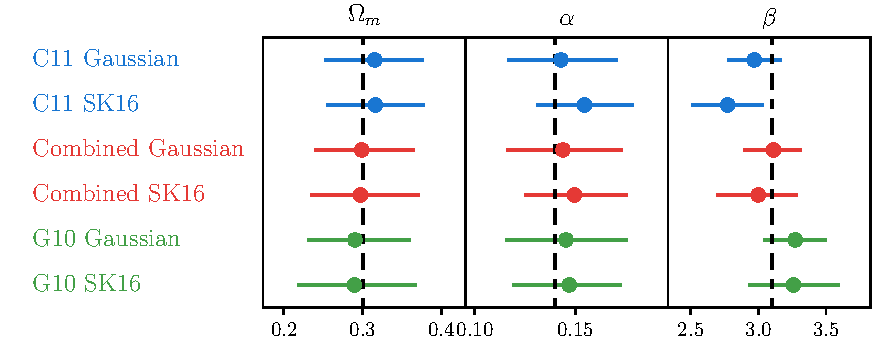
\includegraphics[width=\columnwidth]{approximate_bulk_load_summary.pdf}
	\end{center}
	\caption{Graphical parameter summaries for 150 realisations of supernova data, following Table \ref{tab:bulk_summary}.}
	\label{fig:bulk_summary}
\end{figure}

\begin{figure}
	\begin{center}
		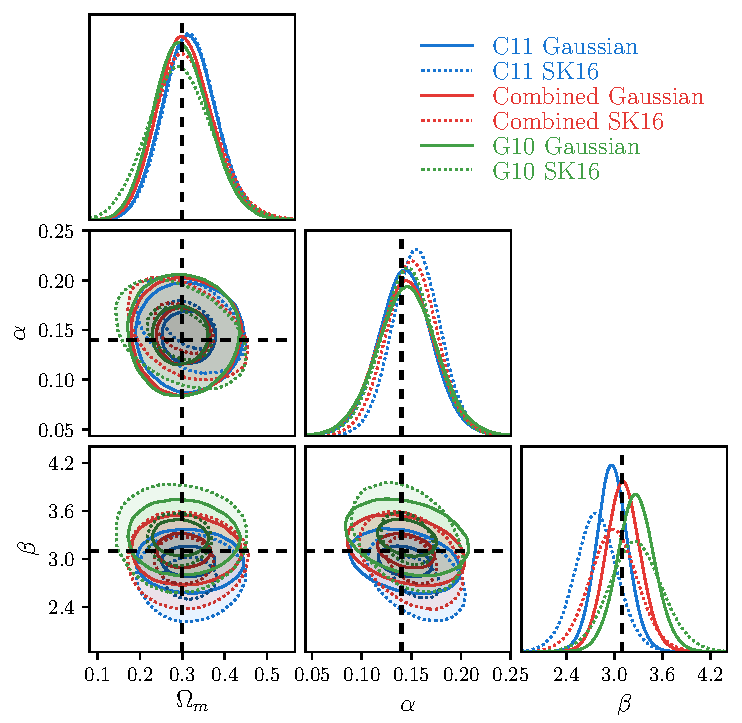
\includegraphics[width=\columnwidth]{approximate_bulk_load.pdf}
	\end{center}
	\caption{Posterior surfaces for 150 realisations of supernova data. Neither population nor scatter model has a significant effect on posterior surface location or shape. Population skewness has the primary effect of changing the degeneracy direction for the $\alpha$ -- $\beta$ contour, whilst the scatter models and skewness have noticeable effects on the value and uncertainty of the recovered parameter $\beta$.}
	\label{fig:bulk_posterior}
\end{figure}





\section{Systematics Strength Test}
\label{sec:sys}

\subsection{Singular Permutations}

To test the impact of various systematics, we generate an array of simulations in which we simulate a dataset with one of the systematic variables permuted. We inspect the effects of systematic shifts using two cosmological models - Flat $\Lambda$CDM and Flat $w$CDM. To make the effects of the systematics more easily seen, we increase our simulated sample size to 500 LowZ and 500 DES-like supernovae, and enforce a prior on $\Omega_m \sim \mathcal{N}(0.3, 0.01)$ on the Flat $w$CDM model. In these test we wish to inspect the shift in statistical uncertainty with simulated systematic effects, and so compare first to a series of simulations with no simulated systematic changes, and also disable our treatment of systematics as described in Section \ref{sec:systreat} for these tests. Our tests are broken down into groups, where systematics of different nature are treated separately. In each simulation, only one systemic is permuted. For a baseleine, our first set has no systematic shift, and so the uncertainty in the parameter summaries is given by statistical uncertainty only. We then test several variations:
\begin{enumerate}
	\item 0.02 Gaussian error on the zero point offsets in a randomly selected band.
	\item $20 \angstrom $ Gaussian error on the filter wavelength.
	\item 10\% Gaussian error in the bias corrected flux measurement (with correct flux uncertainty).
	\item 10\% Gaussian error in the bias corrected flux measurement, but with incorrect flux error.
	\item 20\% Gaussian error on the Milky Way E(B-V) dust correction scale.
	\item 0.2 Gaussian error on the value of $R_V$ for calculating the extinction curve.
\end{enumerate}

\begin{figure}
	\begin{center}
		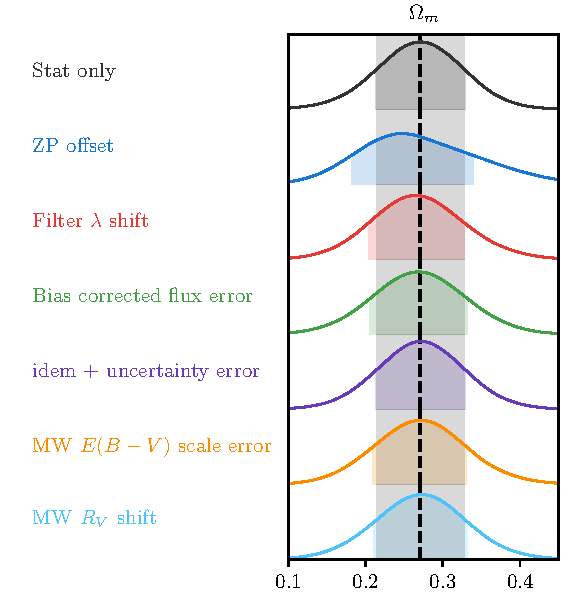
\includegraphics[width=\columnwidth]{approximate_systematic_load_summary.pdf}
	\end{center}
	\caption{Investigating the impact of $\Omega_m$ by systematic permutations under Flat $\Lambda$CDM cosmology, validated using 200 realisations of data, with each dataset containing 500 LowZ supernovae and 500 DES-like supernovae.}
	\label{fig:sys_om}
\end{figure}
\begin{figure}
	\begin{center}
		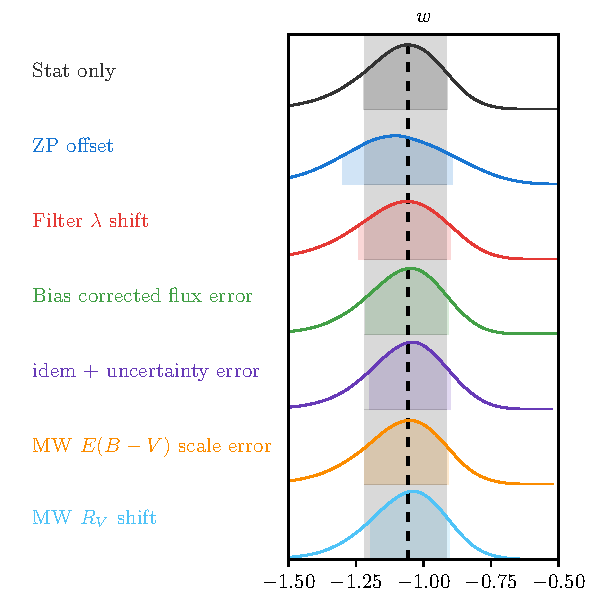
\includegraphics[width=\columnwidth]{approximate_systematic_load_w_summary.pdf}
	\end{center}
	\caption{Investigating the impact of $w$ by systematic permutations under $w$CDM cosmology with the prior $\Omega_m \sim \mathcal{N}(0.3, 0.01)$, validated using 200 realisations of data, with each dataset containing 500 LowZ supernovae and 500 DES-like supernovae.}
	\label{fig:sys_w}
\end{figure}

We find that the most significant systematic are the zero points, as the 0.02 Gaussian error given to them resulted in significant changes to the shape of the marginalised posterior surface for both $\Omega_m$ and $w$, shifting them both to lower values and increasing uncertainty.

{\red What are the actual size of the uncertainties of the systematics? Ie are zps really that badly known? Once I know, I can talk about if any of these are significant.}

\subsection{Full Permutations}

{\red When I have the final sims from Rick I can flesh this out}


\section{DES Forecasts}
\label{sec:forecasts}

To forecast the results for the 3 year DES spectroscopic supernovae sample, we generate 100 realisations of datasets, each comprising 300 low redshift supernovae and 250 DES-like supernovae. We fit these through the three cosmological models - Flat $\Lambda$CDM, $\Lambda$CDM and $w$CDM, however focus mostly on the $w$CDM model as it is the primary scientific concern of the Dark Energy Survey. We run all three cosmological models with systematics enabled and disabled to explicitly show the uncertainty included from systematic contribution.

{\red How to include flat lambdacdm - the plot is boring, just quote the results, or just quote uncertainty, should I round the uncertainty to make it symmetric? Cant do that for wCDM or LambdaCDM because theyre definitely not gaussian}

{\red Talk about how these arent even competitive with JLA and we really need to combine data. Talk about how the photometric supernova dataset should be way better? Talk about statistics limited.}

\begin{figure}
	\begin{center}
		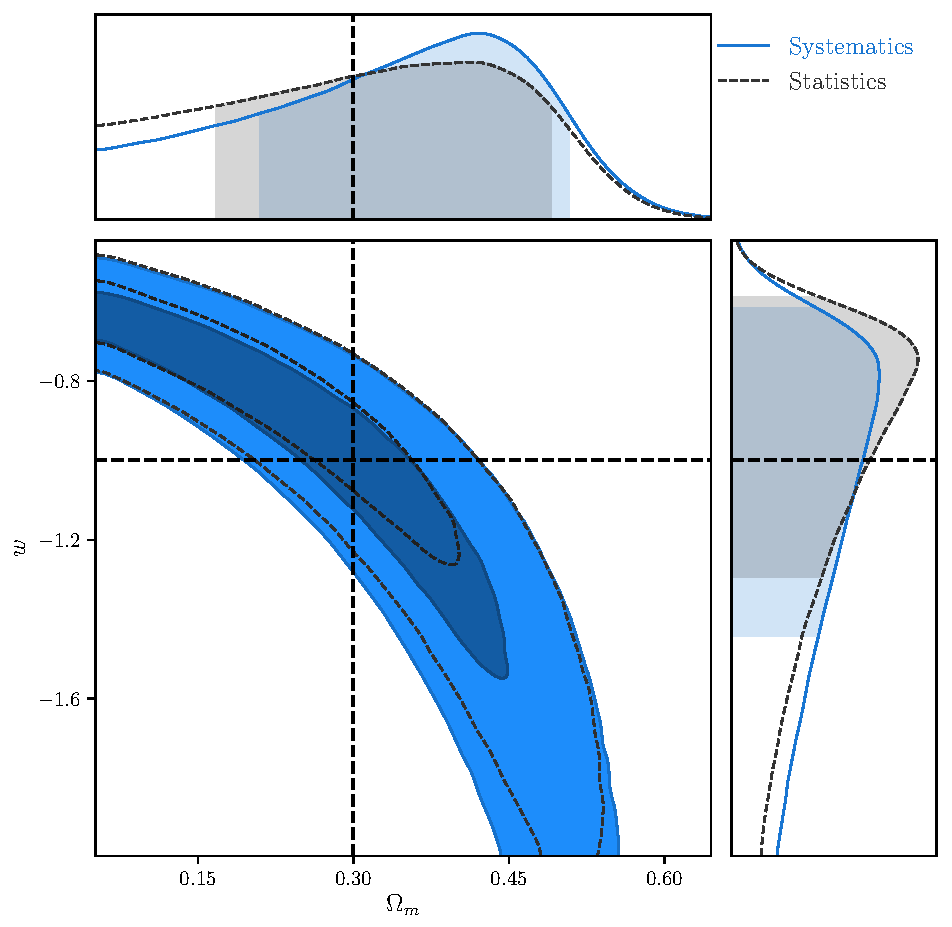
\includegraphics[width=\columnwidth]{combined_ApproximateModelW.pdf}
	\end{center}
	\caption{w.}
	\label{fig:combined_w}
\end{figure}
\begin{figure}
	\begin{center}
		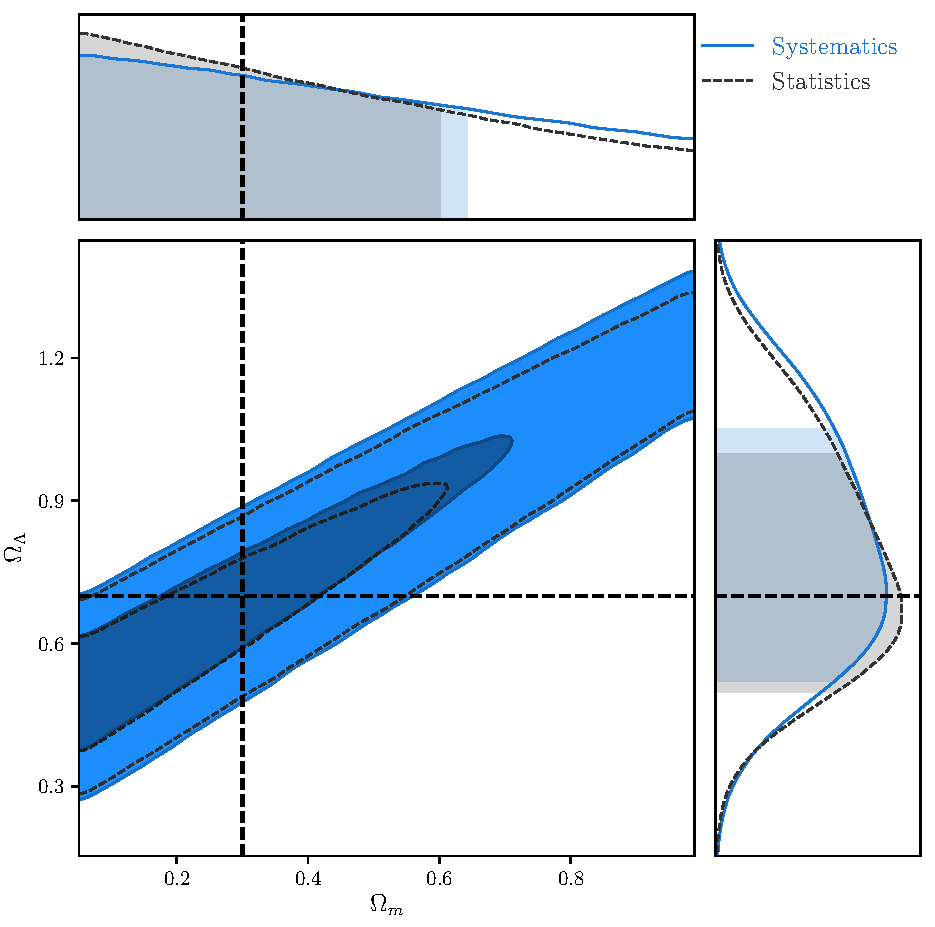
\includegraphics[width=\columnwidth]{combined_ApproximateModelOl.pdf}
	\end{center}
	\caption{ole.}
	\label{fig:combined_ol}
\end{figure}


\section{Conclusions}



\section*{Acknowledgements}

Plots of posterior surfaces and parameter summaries were created with \verb|ChainConsumer| \citep{Hinton2016}.



%%%%%%%%%%%%%%%%%%%% REFERENCES %%%%%%%%%%%%%%%%%%

% The best way to enter references is to use BibTeX:

\bibliographystyle{mnras}
\bibliography{bib}




%%%%%%%%%%%%%%%%% APPENDICES %%%%%%%%%%%%%%%%%%%%%

\appendix

\section{Selection Effect Derivation}
\label{app:selection}




%%%%%%%%%%%%%%%%%%%%%%%%%%%%%%%%%%%%%%%%%%%%%%%%%%


% Don't change these lines
\bsp	% typesetting comment
\label{lastpage}
\end{document}

% End of mnras_template.tex